\section{Introduction}
\label{Chap:Al/Vac:section:Intro}

7000 series Al alloys developed for aerospace applications have high specific strength in the peak-aged condition. Carmakers are exploring options for using stamped 7000 series sheets in structural applications in cars and trucks, from both the manufacturing perspective and the performance perspective. Their widespread implementation in the automotive industry for body and closure applications can achieve vehicle lightweighting goals if the challenges of the component forming and fabrication can be overcome. \cite{fridlyander2002aluminum,hirsch2011aluminium,hirsch2014recent}

\begingroup
\begin{figure}[!ht]
  \centering
  \subfigure{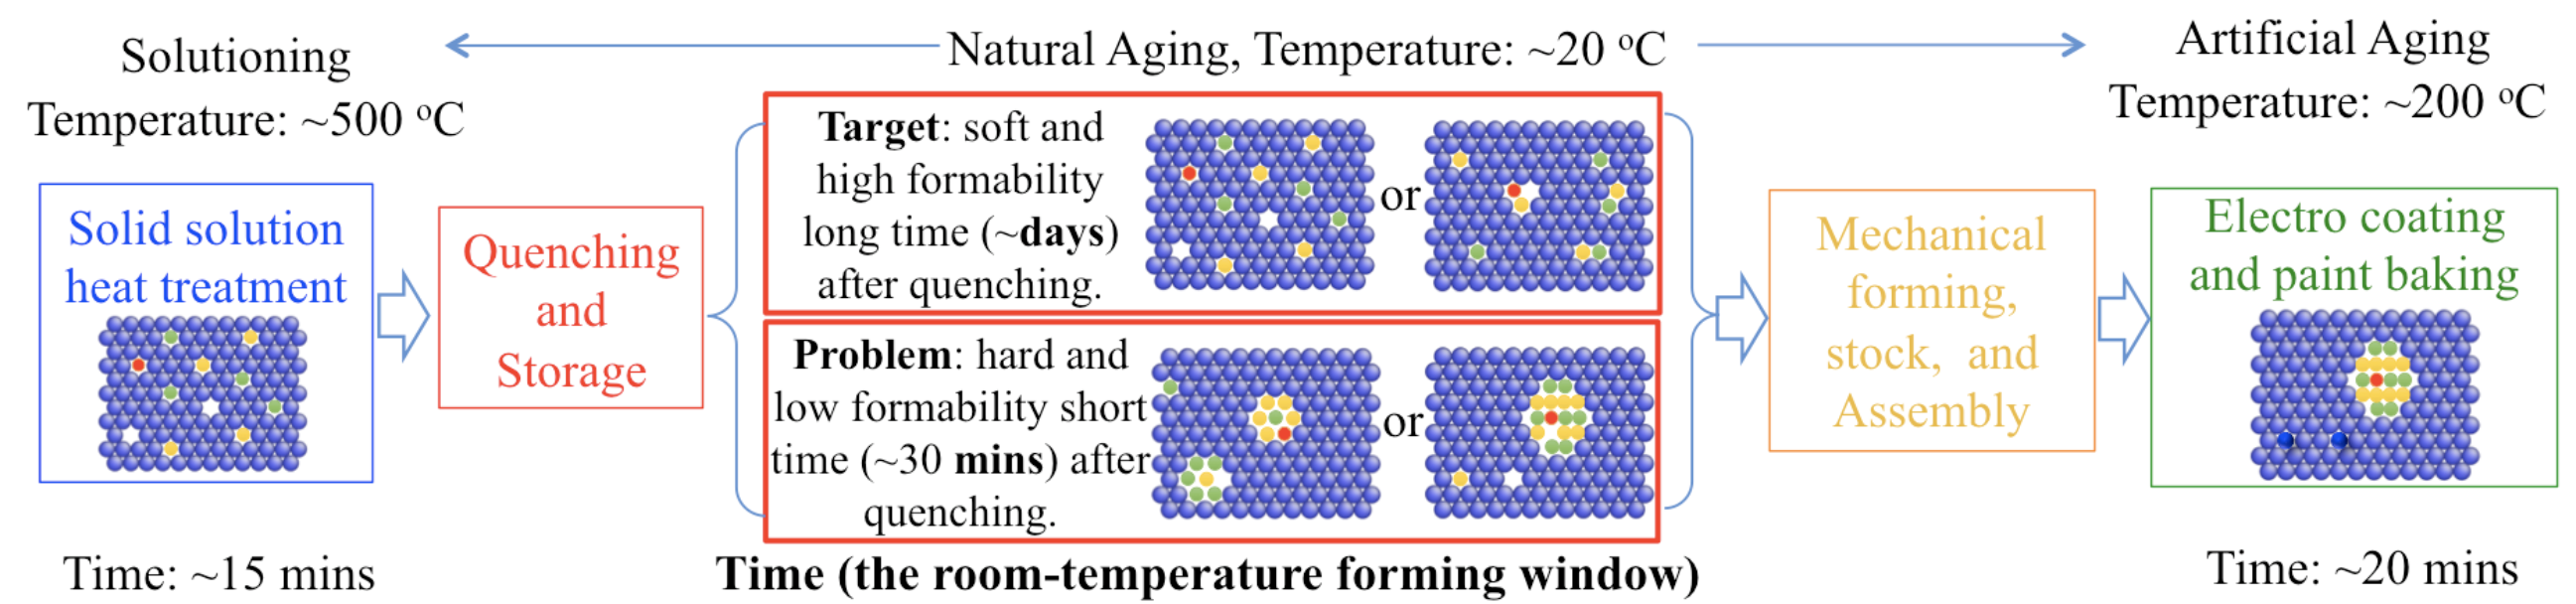
\includegraphics[width=1.0\linewidth]{Chap5/plots/Picture1.png}}
\caption[Schematics of fabrication process of 7000 series Al sheet alloy parts in automobile industry.]{Schematics of fabrication process of 7000 series Al sheet alloy parts in automobile industry. The corresponding changes of illustrated atomistic structures of precipitates during this process are also plotted (blue: Al atoms, other colors: solutes).}
  \label{Chap:Al/Vac:fig1}
\end{figure}
\endgroup

As show in Fig. \ref{Chap:Al/Vac:fig1}, conventional automotive mechanical forming processes such as stamping and hemming, involve room temperature forming of Al sheet alloys in the as-quenched state when alloys have high ductility and formability, followed by artificial aging during the paint bake operation. Due to fast (often within 30 minutes after quenching) and continuously varying natural aging characteristics of current 7000 series alloys, the formability decreases very rapidly and keeps changing as the aging time increases, necessitating costly steps such as warm stamping and coupled solutioning-quenching-stamping operations in a narrow time window. \cite{bryant1999effects,li2004biaxial} These variations of formability and other mechanical properties are all related to the evolution of atomistic structures of precipitates during the sheet processing procedures.

As a result, to understand and to control the nucleation and early stages of precipitation kinetics will have a great impact in automotive applications of age-hardened, light-weight alloys. \cite{deschamps1998influence,banhart2011kinetics,liang2012kinetics,deschamps2014precipitation} The nucleation and growth of precipitates in Al-Zn-Mg-based alloys is currently understood to follow the following sequence: supersaturated solid solution (SSSS) $\rightarrow$ \acf{VRC} $\rightarrow$ \acf{GP} zones (nanoscale coherent Mg/Zn-rich clusters) $\rightarrow$ $\eta'$ (semi-coherent Mg-Zn-Al precipitates with high Zn/Mg ratio) $\rightarrow$ $\eta$ (incoherent $\text{MgZn}_\text{2}$). \cite{ragueneau2000review,deschamps2014precipitation,berg2001gp,chung2018transmission} During natural aging, the majority of precipitates are \ac{VRC} and \ac{GP} zones, even though $\eta'$ can also be found in some cases. \cite{mukhopadhyay1994guinier} Therefore, in this chapter, how to retard the nucleation and growth of \ac{VRC} and \ac{GP} zones in 7000 series Al alloys during natural aging without reversely effects on the precipitation kinetics during subsequent artificial aging will be focused on. To improve upon the predictions of classical theory on the nucleation and early stages of growth of precipitates, atomistic simulations, especially \ac{KMC}, have been applied to investigate the precipitation kinetics in Al alloys. \cite{clouet2006kinetic,soisson2010atomistic,soisson1996monte,liang2012kinetics,sha2005kinetic,clouet2004nucleation,vincent2008precipitation,hirosawa1998comparison,sanchez1984generalized}


As we previously mentioned in Section. \ref{Chap:Mech:NN}, due to the simplicity of analytical formulas and costly \ac{DFT} calculations, empirical potentials can only focus on a limited number of material properties of the fitted system. As the number of species included in the system increases, it is also getting more difficult to fit the desired empirical potential. For simple vacancy-bulk diffusion or surface diffusion events, \acf{BEP} relationship \cite{bronsted1924katalytische, evans1936further, bell1936theory} was commonly used for calculating diffusion barriers:
\begin{subequations}
\begin{align}
E_a = a \Delta E + b
\label{Chap:Al/Vac:eq:BEP}
\end{align}
\end{subequations}
where a, b are weighting parameters from fitting, and $E_a$, $\Delta E$ are the diffusion barrier and the energy difference, respectively. To further simply the calculations, researchers used the bond counting model up to a certain cutoff to estimate the energy differences. \cite{soisson1996monte, soisson2010atomistic} More advanced methods include the \acf{CE} formalism that can consider both pair and triple interactions between neighbors. \cite{sanchez1984generalized,zunger1994statics,van2001first,persson2010lj,natarajan2016early} However, most of the work with \ac{CE} only work efficiently for binary or ternary systems due to high computational costs. \cite{wu2016cluster} Even though with some recent development\cite{nguyen2017cluster}, \ac{CE} can predict energy accurately for quinary alloy systems, this method still oversimplified the contribution of atomistic local environments and elastic energetics. As shown in Fig. \ref{Chap:Al/Vac:fig2}, the correlation between diffusion barriers ($E_a$) and energy differences ($\Delta E$) of Al-Mg-Zn systems is far from linear. This makes the prediction of accurate diffusion barriers very difficult. An inaccurate diffusion barrier could be fatal in \ac{KMC} models. This issue is known as the "small-barrier" issue. \cite{miron2004multiple} Besides, to achieve the same order of accuracy as the number of species increases, the number of parameters needed to fit also increases dramatically\cite{castin2008use}, hence making the computation unaffordable for long time \ac{KMC} simulations.


\begingroup
\begin{figure}[!ht]
  \centering
  \subfigure{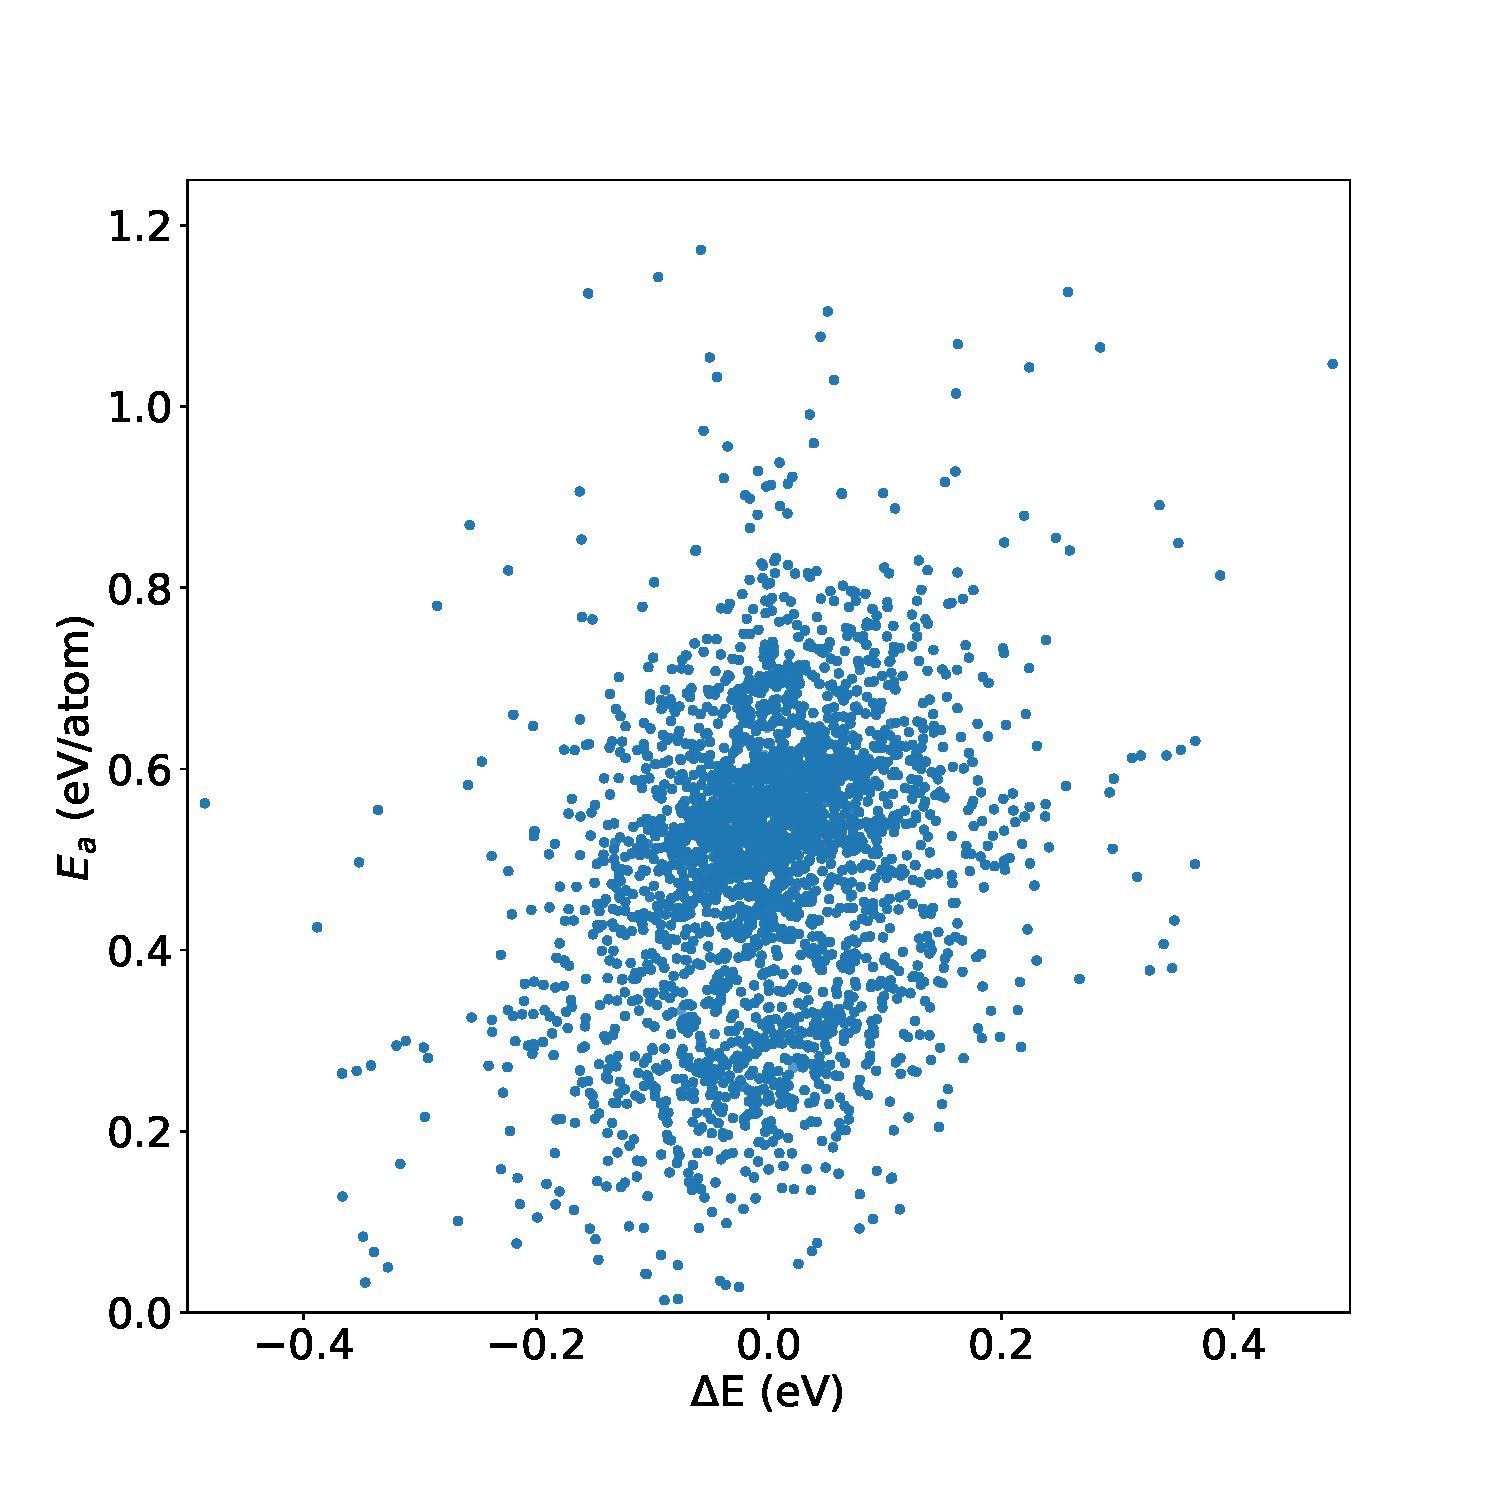
\includegraphics[width=0.8\linewidth]{Chap5/plots/E-EB.pdf}}
\caption[Correlation between diffusion barriers and energy differences for multi-component Al-Mg-Zn systems]{Correlation between diffusion barriers and energy differences for multi-component Al-Mg-Zn systems.}
  \label{Chap:Al/Vac:fig2}
\end{figure}
\endgroup


We will use a machine learning method to predict accurate diffusion barriers for multi-component systems. Recently statistical machine learning and artificial intelligence techniques start to be used in many research fields including materials science and engineering. In general, there are two different approaches to apply machine learning in materials research. One approach is to use machine learning to construct the numerical functions for the interatomic force fields. \cite{bartok2010gaussian,behler2011atom,szlachta2014accuracy,artrith2016implementation,mehta2014exact,artrith2017efficient} Compared with conventional interatomic potentials with fixed mathematical forms, the high flexibility of these machine- learning methods increase the possibility to fit complex potential energy landscapes with enough accuracy at the level needed. In this work, a machine learning method will be used to predict diffusion barriers directly from local atomic structures.


In this chapter, we will first apply first-principles calculations to obtain a training set for diffusion barriers of a single vacancy in various local environments. Then, we will construct machine-learning interatomic potentials for multi-component Al-Zn-Mg systems without/with suggested trace solute elements. These potentials will be used in \ac{KMC} simulations and molecular static/dynamic(MS/MD) simulations to predict the structures/compositions of \ac{VRC}/\ac{GP} zones and their effects on hardness increments during natural aging with the help of phenomenological strengthening models.